\documentclass[twocolumn]{article}
\usepackage[utf8]{inputenc}
\usepackage[version=4]{mhchem}
\usepackage{hyperref}
\usepackage{graphics}
\usepackage{graphicx}
\usepackage{wrapfig}%lässt Textumflossene Bildeinbindung zu
\usepackage{placeins}
\usepackage{enumitem}

\title{Chemistry 2 TP1}
\author{Louis-Hendrik Barboutie}
\date{$2^{nd}$ March 2022}

% ADD CALIBRATION DISCUSSION AND ERROR PROPAGATION

\begin{document}
\maketitle

\onecolumn
\tableofcontents
\twocolumn

\clearpage
\section{Abstract}
The aim of this experiment is to determine an unknown concentration of a HCl solution by using the method of titration with a NaOH solution. After confirming the concentration of the NaOH solution to be $0,1 \ mol \cdot L^{-1}$, it has been found, that the unknown concentration is $0,098 \ mol \cdot L^{-1}$.
\section{Introduction}
The aim of this lab class is to determine the unknown concentration of HCl in an aqueous solution. This will be determined by the method of titration. We will utilize a solution of NaOH as titrant, whose concentration we will beforehand verify using potassium hydrogen phtalate (KHP), by the means of titration as well. We will use the acid-base properties alongside a color indicator to detect when both reactants are introduced in stoechiometric amounts and from there deduce the concentrations.\\
Both a pH-meter and a color indicator will be used. The color indicator lets us visualize easily when both reactants are in stoechiometric proportions, while the pH-meter gives us a numerical value of the pH, allowing us to know how close we are to the equilibrium point.\\
The pH is defined as: pH$=-ln([\ce{H3O+}])$. It measures how acidic or basic a solution is, on a scale of 0-14. Following the Brønsted–Lowry acid-base theory, an acid is a proton (\ce{H+}) donor, and a base is a proton receiver. In an acid-base reaction, an acid and a base react to form either a pH-neutral product, or again an acid and base. Acids and bases are subdivided into "weak" or "strong", referring to their ionizability during the reaction. It is an important property for the precision of the experiment, as strong acids and bases completely react.
\section{Experiment}
\subsection{Chemicals used}
\subsubsection{Water}
Water has a special property: it is "pH-neutral" , ie. it's neither an acid or a base. However, there are still hydronium ions (\ce{H3O+}) and hydroxide ions (\ce{HO-}) present, which form an acid-base couple. \\
Chemical formula: \ce{H2O} \\
pH-neutrality: pH$_{\ce{H2O}}$ = 7
\subsubsection{Sodium hydroxide}
Sodium hydroxide is a strong base. It is used as titrant for both titrations.\\
Chemical formula: NaOH \\
Molar mass: $39.9971 g \cdot mol^{-1}$ [1] 
\subsubsection{Hydrogen chloride}
Hydrogen chloride is a strong acid. It is the chemical contained in the solution of unknown concentration.\\
Chemical formula: HCl\\
Molar mass: $36.46 g \cdot mol^{-1}$ [2]
\subsubsection{Potassium hydrogen phtalate}
KHP is a weak acid. We have a solution of known concentration.\\
Chemical formula: C8H5KO4\\
Molar mass: $204.222 g \cdot mol^{-1}$ [3]
\subsubsection{Phenolphtalein}
Phenolphtalein is a color indicator. It changes color depending on the pH of its environnment.\\
Chemical Formula: \ce{C20H14O4} [4]\\ 
Turning zone: 8,2 - 9,8\\
Colour change: colourless - pink. 
\subsection{Support reactions}
For the first titration, we use the support reaction:
\[ \ce{NaOH + C8H5KO4 -> KNaC8H4O4 + H20} \]
For the second titration, we use the support reaction:
\[ \ce{NaOH + HCl -> NaCl + H2O} \]
Note that for both titrations, when the reactants are introduced in stoechiometric proportions, they will be present in 1:1 ratios (in terms of moles) inside the analyte.
\subsection{Protective equipment}
Since during the experiment we handle irritating and corrosive chemicals, the safety equipment includes safety goggles, nitril gloves and a lab coat.
\subsection{Experimental Setup}
The titrant is always the same solution of NaOH. The analyte will first be a diluted solution of KHP, and in the second titration will be a diluted solution of HCl.
\begin{figure}[!htbp]
    \centering
    \includegraphics[width= 5cm]{Chemistry2_TP1_Setup.jpg}
    \caption{Titration setup}
    \label{fig:1}
\end{figure}
\FloatBarrier
\subsection{Preparation of the analytes}
The analyte solutions for the two experiments were prepared in the following way:
\begin{enumerate}
    \item For the solution containing KHP: \\ A known amount of KHP in solid state was dissolved in some distilled water, and a few droplets of phenophtalein were added.
    \item For the solution containing HCl: \\ A known volume of HCl was introduced in a known volume of distilled water, and a few droplets of phenophtalein were added
\end{enumerate}
Please refer to the results and discussion section for concrete numbers.
\subsection{Experiment execution}
The method of titration consists of adding little amounts of titrant into the analyte solution, and measure any relevant changes. In our case, we proceed by adding titrant in rough steps of $0.5mL$ and record the variations of pH and colour of the analyte solution.\\
We can detect the the reactants have been introduced in stoechiometric proportions by two different methods, by using both a pH-meter and a color indicator. Said color indicator, works by having different colors for different pH environments. Since we are using a strong acid, the jump in the pH is noticeably large. The indicator which we are using is phenolphtaleine, which is colorless in an acidic environment, while being bright purple in a basic environment (pH $\geq 8,2$). This indicator tells us when we have reached or overshot the stoechiometric proportions, but cannot tell us how close we are to that point. The pH-meter will allow us to monitor the variations of the pH in the solution, for every amount of titrant we are adding to the analyte solution. When the pH of the analyte solution reads $\text{pH} = 7$, both reactants are present in stoechiometric ratios, and the solution is pH-neutral.
\subsection{Calibration of the pH-meter}
In order to be able to measure the pH using the pH-meter, it needs to be calibrated first. It is calibrated against two solutions of known pH, one of pH = 4 and one of pH = 7.
\subsection{Calculations}
\subsubsection{Physical relationships}
Since in both titrations, the support reactions yield 1:1 ratios for the reactants, we get:
\[ n_{titrant}=n_{analyte} \] where $n$ is the amount of moles, and $[n] = mol$.
In both titrations $n_{titrant} = n_{NaOH}$, while $n_{analyte, 1} = n_{KHP}$ and $n_{analyte, 2} = n_{HCl}$
We can then deduce the concentration of NaOH with the formula:
\[ [NaOH] = \frac{n_{NaOH}}{V_{NaOH, added}}\]
\subsubsection{Errors}
The error calculation is being done via the classic error determination formulae:
\begin{enumerate}
    \item For additive (or substractive) formulae, of the form \[ X = A + B\] the error is : \[\Delta X = \Delta A + \Delta B\]
    \item for multiplicative (or divisive) formulae of the form \[X = A \cdot  B\] the error ir: \[  \Delta X = X\sqrt{\left(\frac{\Delta A}{A}\right)^2+\left(\frac{\Delta B}{B}\right)^2} \]
\end{enumerate}
While not explicitly shown, all errors are calculated with these formulae and rounded up.
\section{Results and discussion}
\subsection{Verification of the concentration of the NaOH solution}
\subsubsection{KHP solution}
An amount of $m_{KHP}=(2,11 \pm 0,01) \ g$ are diluted with deionized water to form $(100,0 \pm 0,1) \ mL$ of solution. This yields that there are $n_{KHP} = (1,03 \pm 0,01) \cdot 10^{-2} \ mol$ in the solution, and the concentration therefore is [KHP] $= (1,00 \pm 0,01 ) \cdot 10^{-1} \ mol \cdot L ^ {-1}$. \\
A sample of $(10,00 \pm 0,02), \ mL$ is taken to form the analyte solution, which is again diluted with $(30,0 \pm 0,5) \ mL$ of water. In the analyte solution there is therefore $n_{KHP} = (1,0 \pm 0,1) \cdot 10^{-3} \ mol$ of KHP.
\subsubsection{Titration}
For the verification of the given concentration of NaOH we get following graph for the titration:
\begin{figure}[htbp]
    \centering
    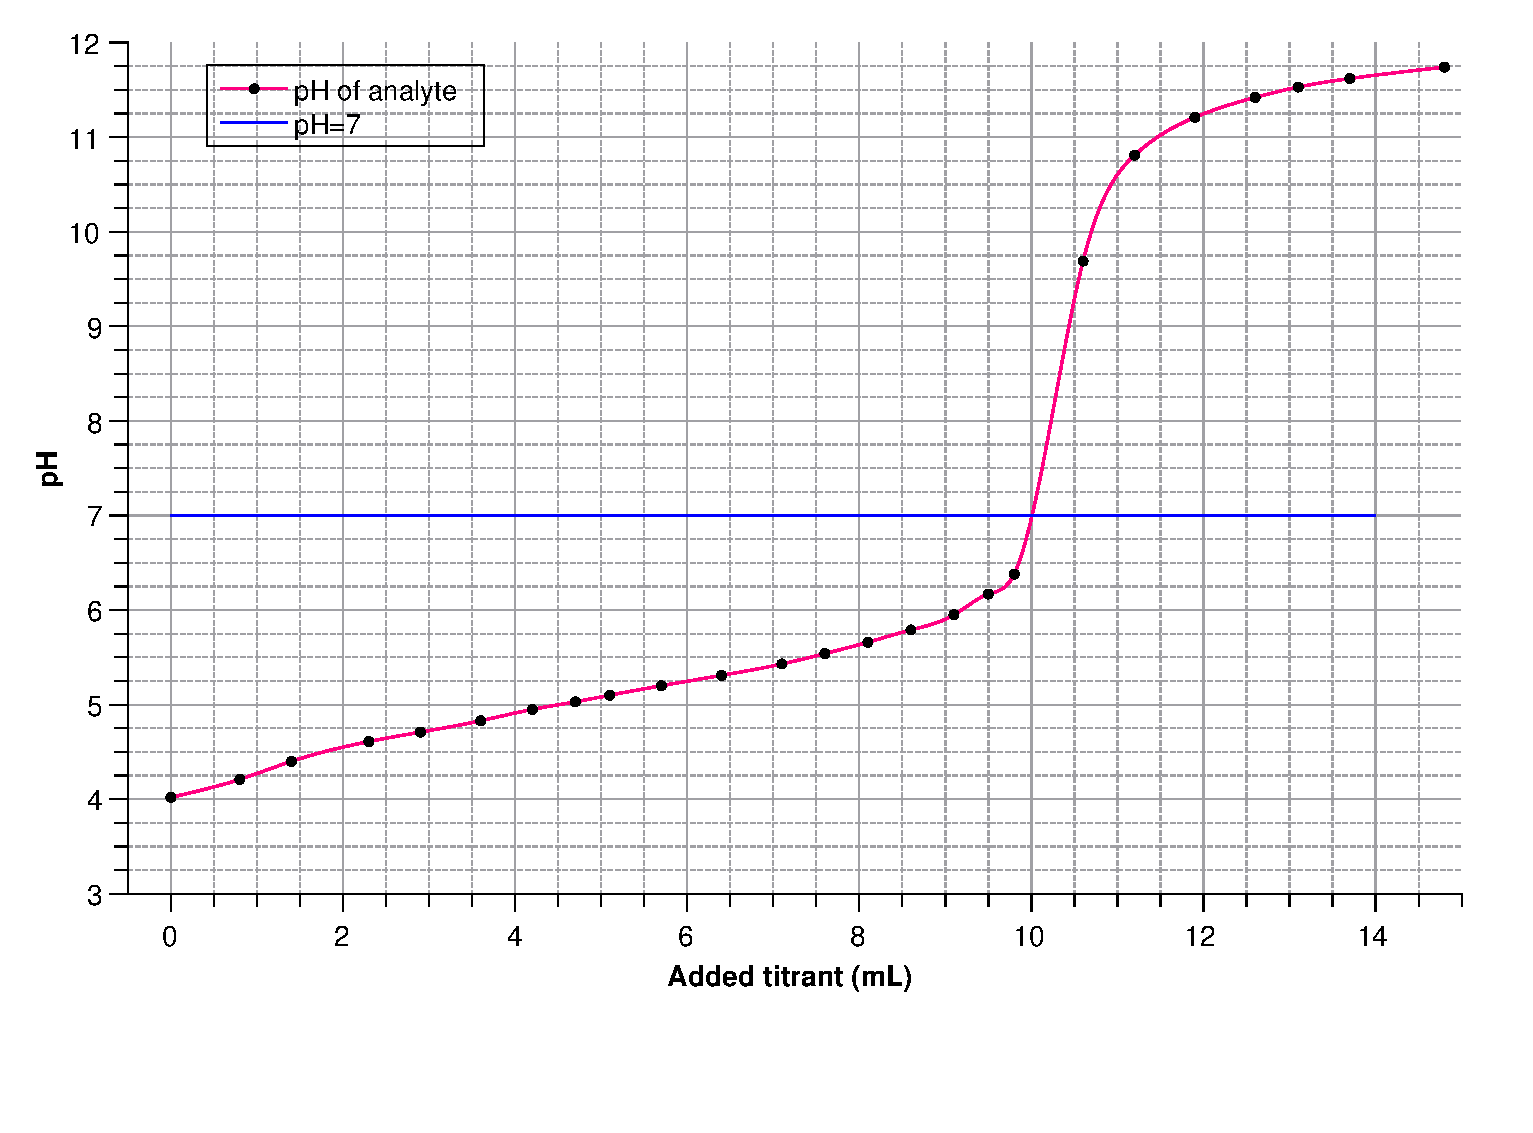
\includegraphics[width=7cm]{Titration1b.eps}
    \caption{Variation of pH in analyte solution with KHP, as function of added volume of titrant containing NaOH}
    \label{fig:2}
\end{figure}
\FloatBarrier
As soon as the jump happens, the color indicator turns bright pink. \\
Using the built-in tool of qtiPlot we get the equivalent volume: $V_{eq} = 10,0 \ mL$, which then yields, using $n_{NaOH} = n_{KHP}$: 
\[ [NaOH]=(0,100 \pm 0,001) \ mol \cdot L ^{-1} \]
Thus confirming the labeling.
\subsection{Determination of the concentration of the HCl solution}
\subsubsection{HCl solution}
The prepared analyte solution contains $30 \ mL$ of deionized water, $10 \ mL$ of the unknown solution and the color indicator. The quantity $n_{HCl}$ is unknown, but we now know the quantity [NaOH].
\subsubsection{Titration}
Repeating the same steps as before, we determine the concentration.    \begin{figure}[!htbp]
    \centering
    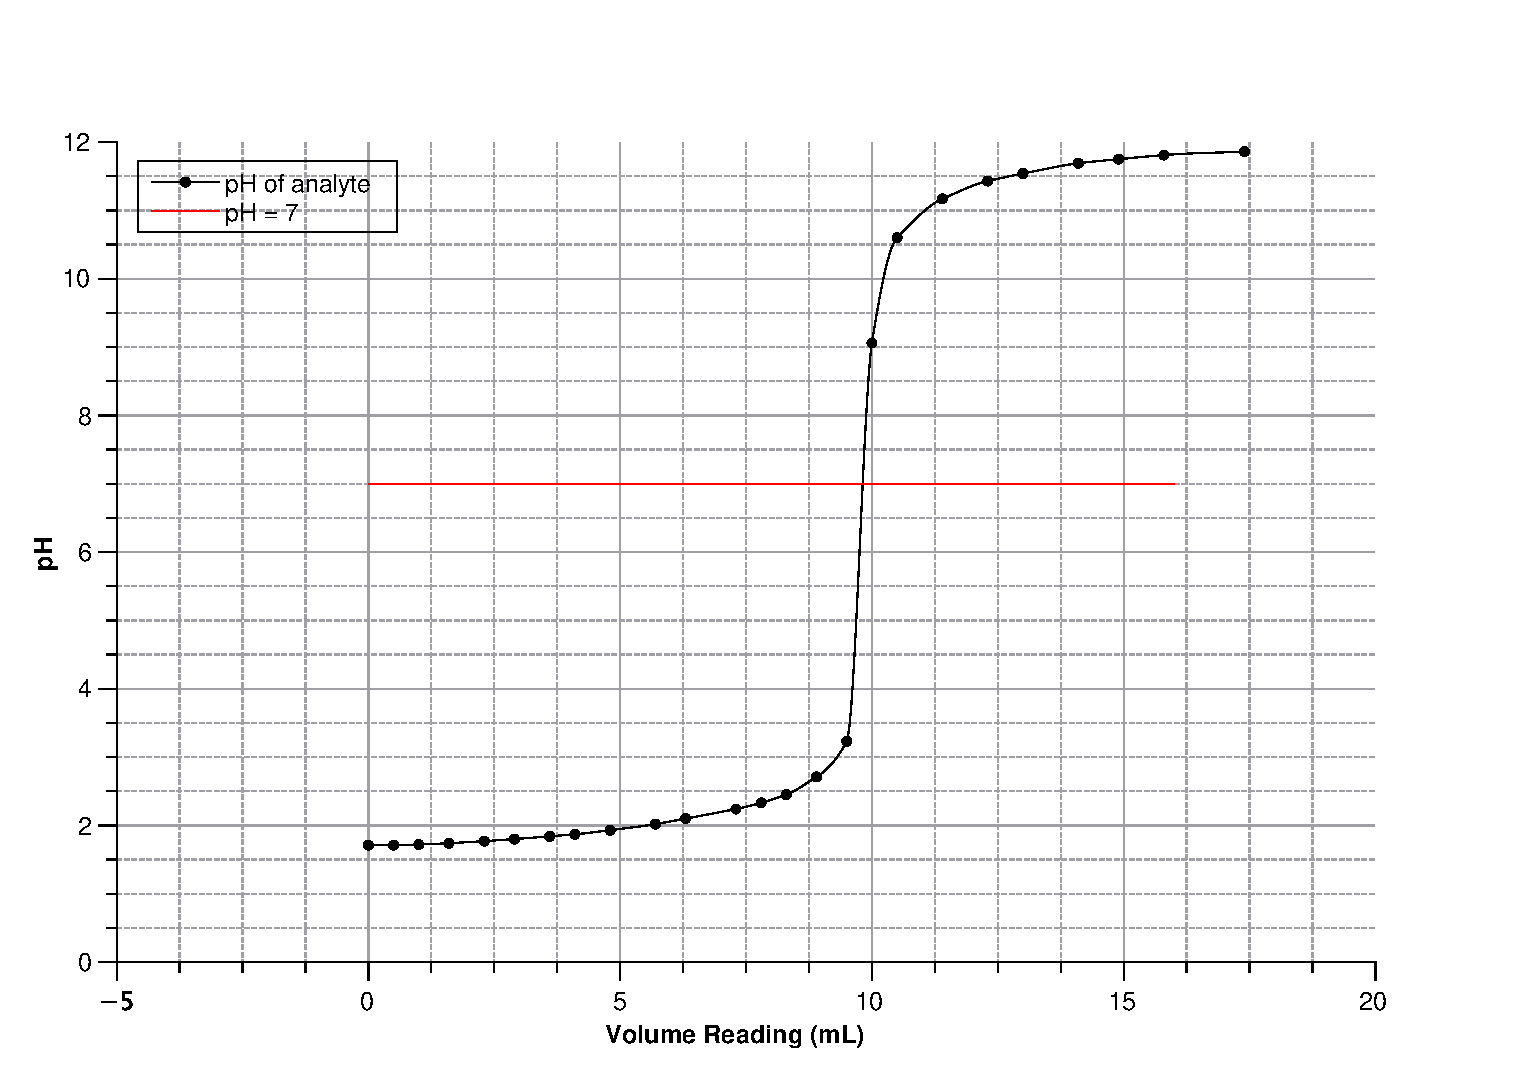
\includegraphics[width=8cm]{Titration2.eps}
    \caption{Variation of pH in analyte solution with HCl, as function of added volume of titrant containing NaOH}
    \label{fig:3}
    \end{figure}
\FloatBarrier
As soon as the jump happens, the color indicator turns bright pink. \\
We deduce with the help of qtiPlot that $V_{eq} = 9,81 \ mL$. Multiplying with the concentration we get:
\begin{align}
    n_{HCl} &= n_{NaOH,added} \nonumber \\
    &=V_{eq} \cdot [NaOH] \nonumber \\
    &= 0,000981 mol \nonumber
\end{align}
Finally, to find the original concentration, we simply need to divide by the sample volume:
\[ [HCl] = \frac{n_{HCl}}{V_{HCl,sample}} = (0,0981 \pm 0,01) \ mol \cdot L^{-1} \]
\subsection{Comparison of both titrations}
We can put both titration curves side by side. We can notice, that for a pH approaching 14, both curves converge. The starting point is different however. It is lower for the HCl solution, since HCl is a stronger acid than KHP.
\begin{figure}
    \centering
    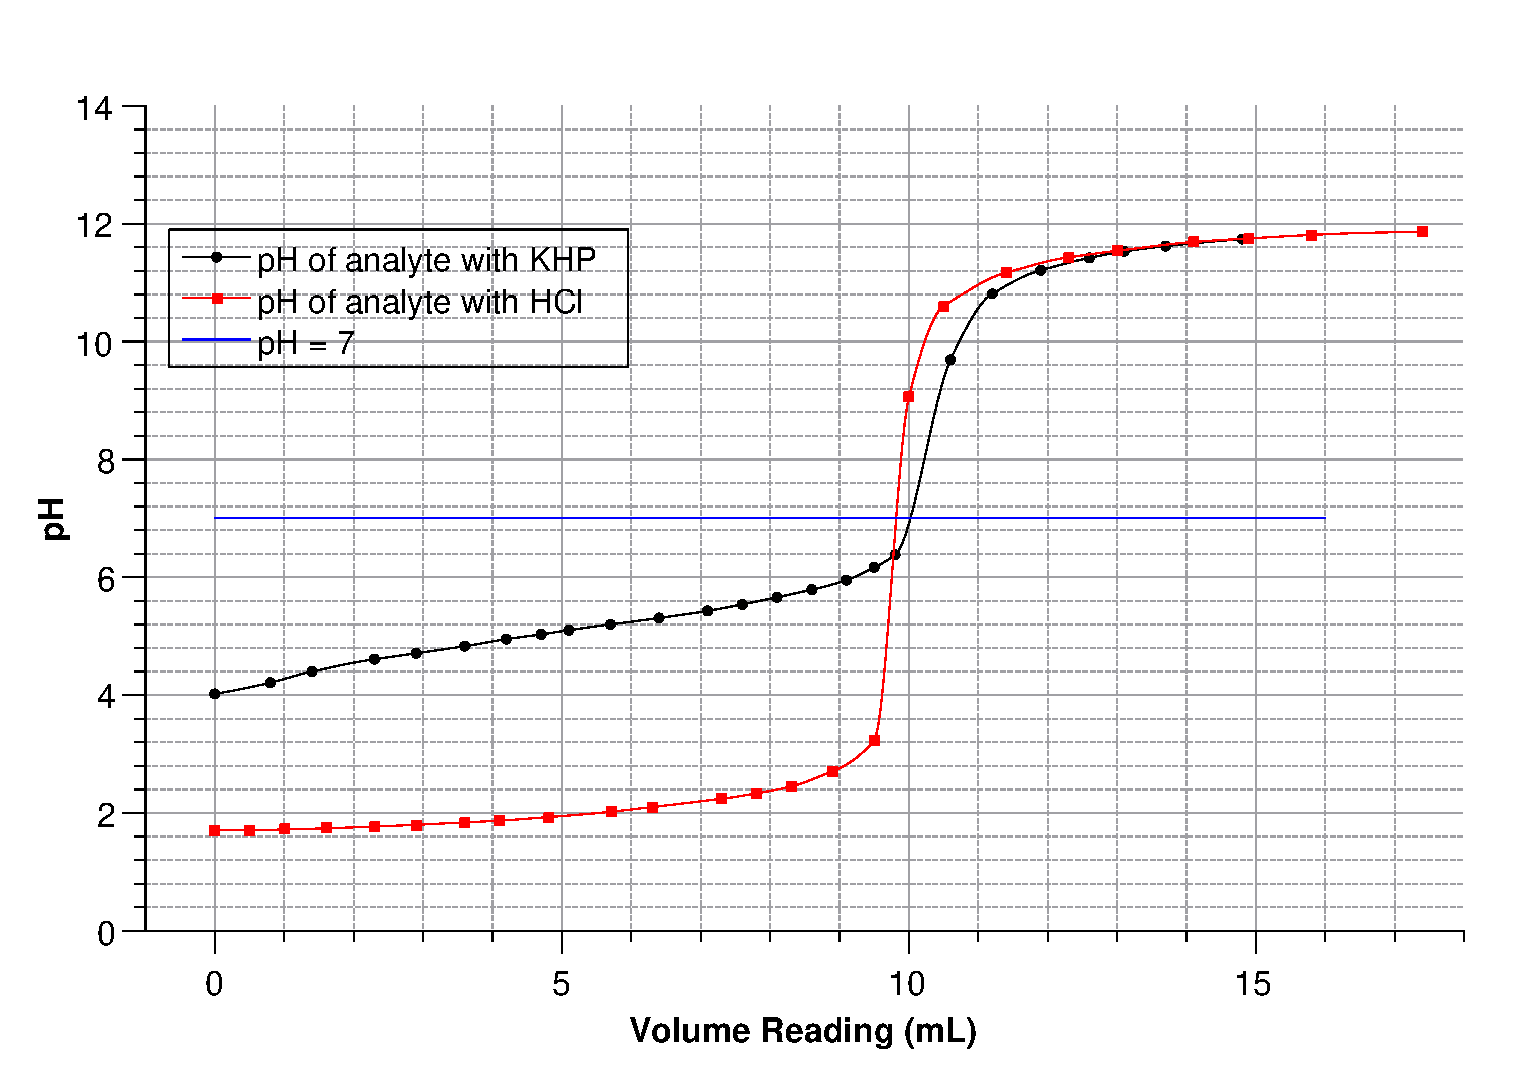
\includegraphics[width=8cm]{Titration1+2.eps}
    \caption{Comparison of both titrations}
    \label{fig:4}
\end{figure}
\FloatBarrier
\subsection{Error estimation}
The error estimates have been inflated to account for bad handling from the operating chemist. While care has been taken to make the most precise readings, some unavoidable errors have occured.
Most notably, the burette, which wasn't completely vertical. The measurement has been always done similarly, and therefore the relative readings of added volume have only minimally been influenced. A big operating mistake, which led to take three times as much acid solution as necessary, and then remove the excess, has also induced additional error (5x as much uncertainty!). Note that the error bars are so small, they aren't visible on the graphs. 
There is also no error given for the determination of $V_{eq}$, as I was unable to identify all sources of error. In fact, the curves have been fitted using the Akima Spline Interpolation Method. Since there is no exact measurement for the pH = 7, the volume reading has an error dependant on the fitting chosen. Furthermore, the first titration features a weak acid, where the pH at the stoechiometric point is not pH = 7, but for simplicity's sake, and because the aim was to do just rough calculations, the method of tangents, which would yield a more precise result, has not been applied. \\
The main sources of error are therefore operating mistakes, but the instrumental errors can be decreased by doing more precise measurements, with more precise hardware \textit{and} software.
\section{Conclusion}
The unknown concentration has been determined to be:
\[ [HCl] = \frac{n_{HCl}}{V_{HCl,sample}} = (0,01 \pm 0,01) \ mol \cdot L^{-1} \]
The experiment could've been improved with a better burette, which would've allowed for finer measurement, especially in the jump zone.
\section{Bibliography}
\text{[1]} \href{https://en.wikipedia.org/wiki/Sodium_hydroxide}{Wikipedia} \\
\text{[2]} \href{https://en.wikipedia.org/wiki/Hydrogen_chloride}{Wikipedia} \\
\text{[3]}\href{https://en.wikipedia.org/wiki/Potassium_hydrogen_phthalate}{{Wikipedia}} \\
\text{[4]} \href{https://en.wikipedia.org/wiki/Phenolphthalein}{{Wikipedia}}
\end{document}